
Two grain geometries were explored: spherical grains and irregular grains. The model assumptions described in this chapter apply to both the spherical and irregular grain models. If there is a slight difference, it will be specified. 

Spherical dust grain modelling is a more common approach the scattering properties of spheres have simpler calculations. The scattering properties for spherical grains were calculated using the DSHARP Mie-Opacity Library (\texttt{DSHARP}) from \cite{dsharp_code}. 


Irregular grains were tested as they are a more realistic shape for dust grains in disks \citep{Lin2024}. The more complicated irregular grain shape affects the scattering properties, making the calculations more difficult and computationally expensive. However, these calculations have become more accessible with \texttt{glitterin} (dust Grain LIght scaTTERIng Neural network) from \cite{glitterin}. Figure \ref{fig: glitterin_dust_grains} shows an example of six irregular grain shapes from \texttt{glitterin}.


\begin{figure}[htbp]
  \centering
  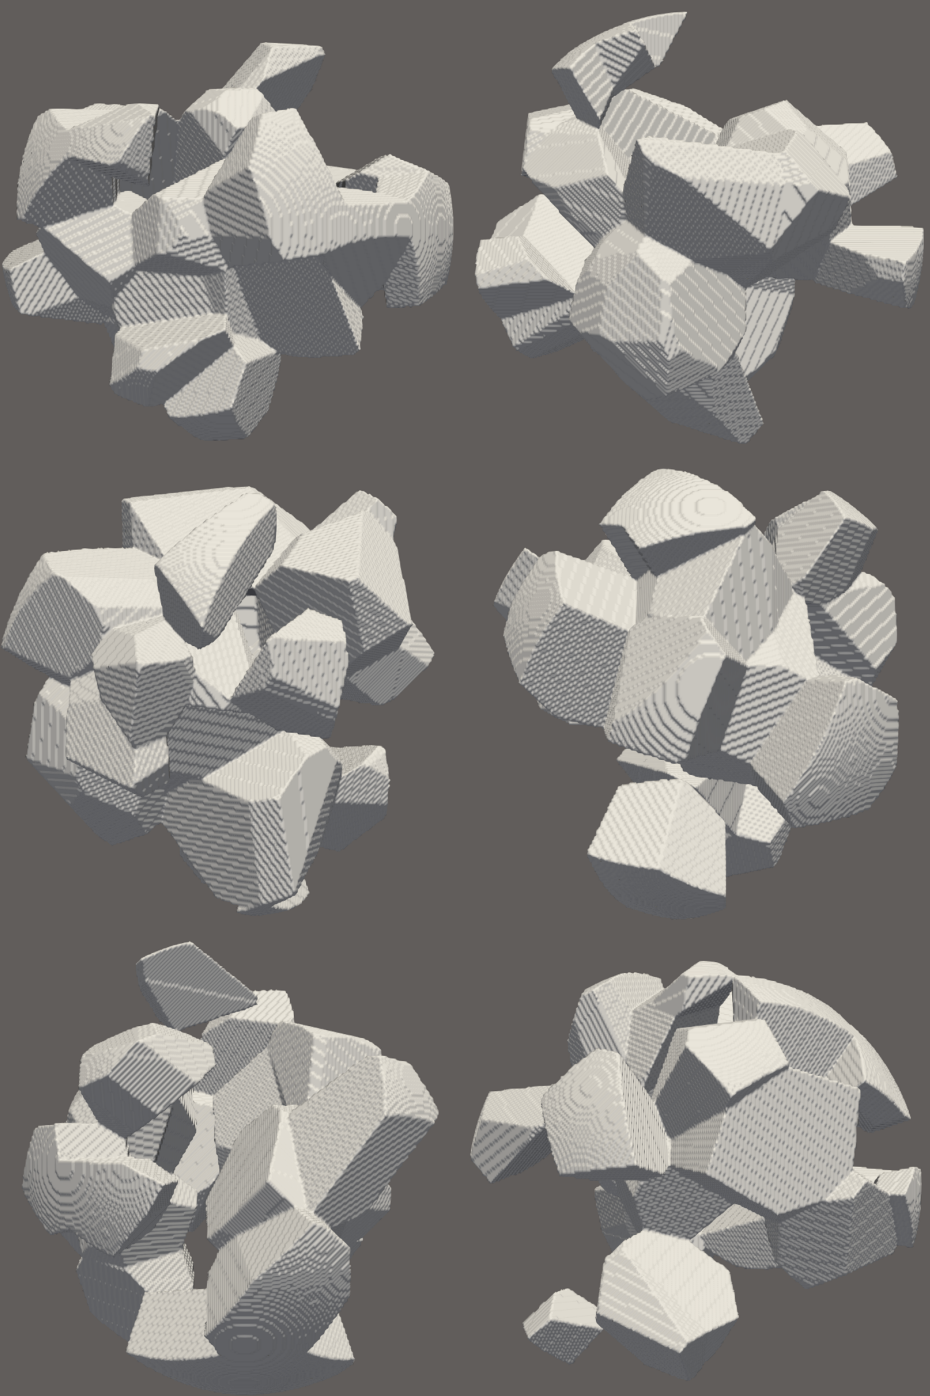
\includegraphics[width=0.3\textwidth]{WRITEUP_AND_IMAGES/IMAGES/WRITEUP/NOTMINE/glitterinFigure1.png}
  \caption[Example of six irregular particles from \texttt{glitterin}.]{Example of six irregular particles from \texttt{glitterin}. Figure from \cite{glitterin}. \permission{ask for permission} }
  \label{fig: glitterin_dust_grains}
\end{figure}
 
 





